\chapter{Open Data -- An Overview}
\label{chap:opendata}

Open data is currently a very popular concept.
As discussed in the previous chapter, it is part of an important political debate related to transparency, citizen participation, and considered a crucial way for improving democracies around the world.
In this chapter, we drive an overview about open data, with the objective of historically contextualizing open data, highlighting the problems and challenges currently observed.
Being a very dynamic field, it is impossible to picture the open data field only looking at academic works.
Thus, the material used to write this chapter also includes websites, practitioners reports and official documents, seeking to reflect more clearly the current open data landscape.
Rather than exhausting the topic, the aim of this chapter is to justify the importance of open data, present the open research issues and point the solutions to be presented in the following chapters.

The chapter starts with a section dedicated to the alleged motivations for opening data, including other contexts than government.
In the sequel, some historical notes about the open concept and the open data term are presented, followed by a collection of open data definitions.
Section \ref{sec:opendatalandscape} reviews the efforts to map the open data landscape using different assessment methods.
In order to ground the discussion in a more concrete basis, in the following section we selected one special type -- open budget data -- to describe in a more detailed fashion.
The chapter continues with two sections that seek to evaluate the results of open data efforts: impacts evaluation (Section \ref{sec:impacts}) and value creation (Section \ref{sec:value}).
Of crucial importance is Section \ref{sec:problems}, where the problems of open data are analysed.
This section is following by the presentation of the Linked Data approach, which is regarded as a way to overcome some of the mentioned impediments.
We finally conclude this chapter pointing selected references to a broader understanding of open data. 

\section{Why Open Data?}
\label{sec:why}

There are several motivations on why one should publish open data.
When data is related to government, and thus called Open Government Data (OGD), reasons are even stronger, because it deals essentially with data related to public administration.
According to the \href{http://opengovernmentdata.org/}{Working Group on Open Government Data} at the Open Knowledge Foundation, there are three main motivations for governments to publish open data:

\begin{itemize}
	\item Transparency;
	\item Releasing social and commercial value; and
	\item Participatory Governance.
\end{itemize}

The same organization curates a collaborative web book which presents a more extensive list of activities possibly benefiting from open government data~\cite{OpenKnowledgeFoundation2015}:

\begin{itemize}
    \item Transparency and democratic control;
    \item Participation;
    \item Self-empowerment;
    \item Improved or new private products and services;
    \item Innovation;
    \item Improved efficiency of government services;
    \item Improved effectiveness of government services;
    \item Impact measurement of policies; and
    \item New knowledge from combined data sources and patterns in large data volumes.
\end{itemize}

A comparison between open government data implementation strategies in 5 countries driven by~\citeonline{Huijboom2011} concluded that there are three primary motivation for governments to publish open data:

\begin{itemize}
	\item Increasing democratic control and participation;
	\item Foster service and product innovation; and
	\item Strengthen law enforcement.
\end{itemize}

Although very important, government data is not only kind of data possible to be opened.
Another important field where open data is discussed is science.
According to~\citeonline{Murray-Rust2008}, copyright over scientific data ``is a major impediment to the progress of scholarship in the digital age.''
His work severely criticizes publishers who impose barriers to free use of academic papers and associated supporting information, such as datasets, experiments data, simulation source code or software output.
The author strongly defends an Open Access policy for publishing scientific work, and also lists a number of reasons why scientific data should be open:

\begin{itemize}
	\item  ``Data belong to the human race.'' Typical examples are genomes, data on organisms, medical science, envi- ronmental data;
	\item Public money was used to fund the work and so it should be universally available;
	\item It was created by or at a government institution (this is common in US National Laboratories and government agencies)
	\item Facts cannot legally be copyrighted;
	\item Sponsors of research do not get full value unless the resulting data are freely available;
	\item Restrictions on data re-use create an anticommons;
	\item Data are required for the smooth process of running communal human activities (map data, public institutions); and
	\item In scientific research, the rate of discovery is accelerated by better access to data.
\end{itemize}

\section{Historical Notes}

Although the idea was present in the scientific world for a long time, the term open data appeared for the first time in 1995, regarding the opening of geophysical and environmental data in an American scientific agency~\cite{Chignard2013}. 
\citeonline{Tauberer2014} also affirms the roots of open data praxis come from the scientific community, who first realized the importance of opening and sharing data.
He affirms that open government data, in turn, ``has its own history rooted in Web 2.0, political campaigns, and innovations inside of municipal governments.''

The open source software movement fights since the 1980's for the source code of software to be open and free\footnote{Richard Stallmann always remembers that `'free'' has the sense of ``free speech'', and not the sense of ``free beer''. However, we must remember that a free beer in the sense of free speech (where the recipe is freely shared) also exists, available at~\url{http://freebeer.org/}.}.
However, with the popularization of the Web, the increased speed in transmission rates, and the widely spread concept of Web Application, it was recognized that opening the source code was not enough for the unrestricted flow of knowledge through the Web.
It was necessary that, beyond the code, public data could also be open, and also considered a common good, a thus not subject to private appropriation.

According to~\citeonline{Chignard2013}, in 2007, a meeting between thinkers and activists in Sebastopol, USA, defined some concepts about open data, and some strategies in order to effectively apply it.
The basic idea is that public data are of common property, as well as in the scientific world.
%%%TODO review this paper

The first days of year 2009 watched the release of a Memorandum on Transparency and Open Government~\cite{Obama2009} by the newly elected administration of Barack Obama, in the USA.
The memorandum is a political commitment on transparency, public participation, and collaboration, stating that ``Openness will strengthen our democracy and promote efficiency and effectiveness in Government''.
On the same year USA and UK released their open data portals in order to centralize the distribution of open government data.
This action was followed by several countries and local administrations, as we will see in Section~\ref{sec:opendatalandscape}. 

The first academic papers about open data started to be published only in 2010, according to a survey driven by~\citeonline{Attard2015}. One year, in 2011 the Open Government Partnership (OGP) was launched by eight countries, aiming to be a platform for national governments to willing to be more open, accountable, and responsive\footnote{Available at~\url{http://www.opengovpartnership.org/}}. In 2015, 69 countries were taking part on it and implementing their 1st, 2nd or 3rd action plans.

Another important historical milestone was the signature of the Open Data Charter\footnote{Available here:~\url{http://opendatacharter.net/}} by the G8 leaders, in 2013. The charter is based on six principles to be followed the governments that adopt it:

\begin{itemize}
	\item Open by Default;
    \item Timely and Comprehensive;
    \item Accessible and Usable;
	\item Comparable and Interoperable;
    \item For Improved Governance and Citizen Engagement; and
    \item For Inclusive Development and Innovation.
\end{itemize}

In 2014, the charter was launched to the G20 group, and in 2015, it was also discussed at the Climate Conference, in Paris.
According to the Open Data Charter portal, only a few countries already adopted it: Mexico, Uruguay, Chile, France, Italy, UK, Philippines, Guatemala and South Korea.

%open data conference?

\section{Definitions}
\label{sec:definitions}

One of the most used and accepted definitions of OGD are the Eight Principles of Open Government Data\footnote{Available at \url{https://opengovdata.org/}}, published as a result of the 2007 Sebastopol experts meeting. The eight principles are: 

\begin{enumerate}
	\item Complete: All public data is made available. Public data is data that is not subject to valid privacy, security or privilege limitations. 
	\item Primary: Data is as collected at the source, with the highest possible level of granularity, not in aggregate or modified forms. 
	\item Timely: Data is made available as quickly as necessary to preserve the value of the data. 
	\item Accessible: Data is available to the widest range of users for the widest range of purposes. 
	\item Machine processable: Data is reasonably structured to allow automated processing. 
	\item Non-discriminatory: Data is available to anyone, with no requirement of registration. 
	\item Non-proprietary: Data is available in a format over which no entity has exclusive control. 
	\item License-free: Data is not subject to any copyright, patent, trademark or trade secret regulation. Reasonable privacy, security and privilege restrictions may be allowed. 
\end{enumerate}

From this definition, it should be noted that several dimensions of data publishing are tackled.
The first three principles are about the \emph{nature of data}, i.e., aspects related to the content represented by data.
The next three ones are about \emph{access to data}, dealing with aspects that impact the technical use abiliy of data.
Finally, the last two principles deal with \emph{legal framework over data}.
However, there is a possible ambiguity on the last principle.
The term \emph{License-free} can be understood both as \emph{free of license}, i.e., there is no legal framework regulating what can and what cannot be done with data, or as possessing a \emph{free license}, i.e., a defined legal framework which guarantees that data is open. 
Nowadays, there is a certain consensus that the latter interpretation is the most productive, since it gives legal parameters for people wanting to re-use data, including for commercial purposes.
Thus, some countries defined their own Open Data Licenses, e.g. Germany\footnote{Available at \url{https://www.govdata.de/dl-de/by-1-0}} and UK\footnote{Available at \url{http://www.nationalarchives.gov.uk/doc/open-government-licence/version/3/}}.
The Open Data Commons platform\footnote{Available at \url{http://opendatacommons.org}.} offers legal support for open data and defines three types of license: Public Domain Dedication and License (PDDL), Attribution License (ODC-By), and Open Database License (ODC-ODbL).

To these 8 principles, another 6 ones were added by~\citeonline{Tauberer2014}:

\begin{enumerate} \setcounter{enumi}{8}
	\item Permanent: Data should be made available at a stable Internet location indefinitely.
	\item Safe file formats: “Government bodies publishing data online should always seek to publish using data formats that do not include executable content.”
	\item Provenance and trust: “Published content should be digitally signed or include attestation of publication/creation date, authenticity, and integrity.”
	\item Public input: The public is in the best position to determine what information technologies will be best suited for the applications the public intends to create for itself.
	\item Public review
	\item Interagency coordination
\end{enumerate}

Another widely accepted definition comes from the general Open Definition, which is currently on version 2.1\footnote{Available at \url{http://opendefinition.org/od/2.1/en/}}.
In contrast to the previous definition, this one is not aware from aspects related to the nature of data, probably because it was originally formulated for open source software, but is currently being applied for data and art works, among others. 
Access to data (e.g., Machine Readability and Open Format) and legal framework (Open License or Status) are covered by this definition.
One advance of the Open Definition is the characterization of conditions that limits the open criteria, such as Attribution (require distributions of the work to include attribution of contributors, rights holders, sponsors, and creators), Integrity (modified versions of a licensed work should carry a different name or version number from the original work) and Share-alike (distributions of the work should remain under the same license or a similar license).

In order to help publishers in creating a roadmap towards open data,~\citeonline{Berners-Lee2010} proposed a five stars schema, where each star represents one step further in turning data more accessible.
The scheme starts from a simple PDF file and finishes with the implementation of the Linked Open Data paradigm (see more Section~\ref{sec:LOD}).
The key elements for each of the five stars are:

\begin{enumerate}
	\item Open License
	\item Machine Readable
	\item Open Format
	\item Dereferenceable URIs
	\item Linked Data
\end{enumerate}

Though not so much cited, the Three Laws of Open Government Data developed by \citeonline{Eaves2009} has the advantage of being written in a colloquial way, supposedly more accessible for non-experts:

\begin{enumerate}
	\item If it can't be spidered or indexed, it doesn’t exist
	\item If it isn’t available in open and machine readable format, it can’t engage
	\item If a legal framework doesn’t allow it to be repurposed, it doesn’t empower
\end{enumerate}

Finally, the Open Data Institute defines a Data Spectrum, which ranges from closed, through shared until open data. Figure~\ref{fig:data_spectrum} pictures this definition.

\begin{figure*}[ht]
\begin{center}
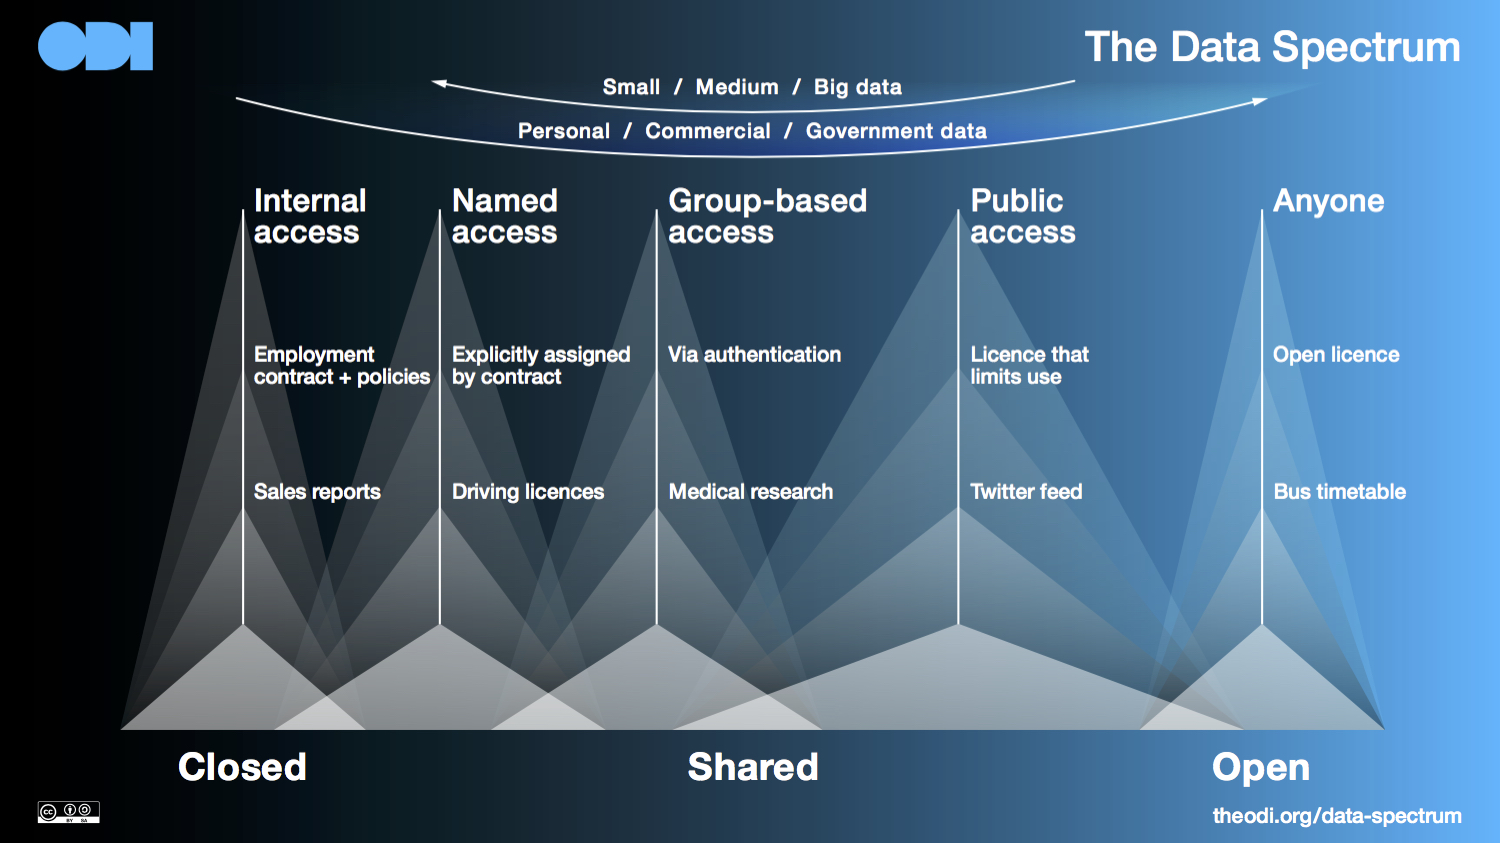
\includegraphics[scale=0.3]{images/odi_open_data_spectrum.jpg}
\caption[Data Spectrum as a definition of steps between open and closed data.]{Data Spectrum as a definition of steps between open and closed data. Source: \url{https://theodi.org/data-spectrum}}
\label{fig:data_spectrum}
\end{center}
\end{figure*}

With the same idea of defining intermediate levels of data openness, \citeonline{Bargh2016} proposed the Semi Open-Data Paradigm.
The objective is the analyse the dissemination of data through several dimensions, as publicity, completeness, timeliness, metadata, and other.
For each dimension, several level should be defined.
On the publicity dimension, the proposed levels are: ‘share with no one’, ‘share data within a specific group’, ‘share data within a department of an organization’, ‘share data within an organization /ministry’, and ‘share data among a federation of organizations’ and finally ‘share with the public’.

%######################################################################
\section{Open Data Landscape}
\label{sec:opendatalandscape}

While the number of open data initiatives around the world increases dramatically every year, several research projects driven from academy and/or civil society organizations seek to map the open data landscape.
In the following, some of these projects are summarized, and their main results are presented:

\textbf{\href{http://index.okfn.org/}{Open Data Index}:} The Open Data Index is one of the most important platform for analysing the open data landscape in the world. In 2013, the first year, Open Data Index analysed 60 countries. In 2014 this number grew to 97, and in 2015 the evaluation covered 122 countries.
The methodology consists basically in analysing datasets from 13 categories: 
National Statistics, Government Budget, Legislation, Procurement tenders, Election Results, National Map, Weather forecast, Pollutant Emissions, Company Register, Location datasets, Water Quality, Land Ownership and Government Spending.
For each category, 9 features are evaluated with yes or no answers: ``Openly licensed?'', ``Is the data machine readable?'', ``Is the data available for free'',  ``Available in bulk?'', ``Is the data provided on a timely and up to date basis?'', ``Is the data available online?'', ``Is data in digital form?'', ``Publicly available?'' and ``Does the data exist?''.
From this analysis, a ranking is constituted according to each countries \emph{score}. 
This score is a weighted sum that reflects the performance of each category for each feature.
Considering all the countries, only 9\% of the datasets are open. 
However, a strong inequality between the countries can be seen: while 25 of them have 50\% or more datasets open, 44 have less than 25\%.

\textbf{\href{http://www.opendatabarometer.org/}{Open Data Barometer}:} The Open Data Barometer also focus on a comparison of the open data context between countries. However, a more complex methodology is used to analyse each country, including expert interviews and secondary data, apart from accessing the datasets in a similar way as the Open Data Index.
The 2nd Edition of this research, released in January 2015, analysed 86 countries concluded that ``there is still a long way to go to put the power of data in the hands of citizens''\cite{Davies2015} .

\textbf{\href{http://opendatamonitor.eu/}{Open Data Monitor}:} The Open Data Monitor is focused on looking at datasets from European countries. One interesting aspect of this project is the measurement of ``availability'', which considers the existence of ``a description, at least one resource with a functional link and an available email of the author'' for datasets in a catalogue.
Surprisingly, the first three countries with more datasets (Germany, UK and Spain) have only a bit more than half of their datasets available (51\%, 63\%, 57\%, respectively).

\textbf{\href{http://opendatainception.io/}{Open Data Inception}:} This project presents the largest geotagged listing of open data portals, with more than 1600 ODPs showed in a map. For each portal, URL and associated geographical region is given.

\textbf{\href{http://right2info.org}{Right2Info}:} This platform monitors FOIAs, which is not specifically open data, but is very related. 93 countries have some kind of FOIA, and the platform presents a comprehensive list of 273 FOIAs covering various scopes~\cite{Vleugels2012}.

\section{Open Budget Data}

From all types of OGD, one is of particular importance: government budgetary data, as timely access to these data is critical to accomplish government accountability.

All governments and public administrations maintain budgetary data, unlike, for example, bus position data, which depends on sensors, or data about the occurrence of a specific disease, which depends on a health information system.
From the citizen side, information on budget is a key element to ensure that public funds are being properly used.
In locations where a participatory budget~\cite{Mkude2014} was implemented, that is, part of the budget allocation is decided by the community, access to this kind of data is indispensable.
A global initiative to improve openness of governments -- the Open Government Partnership (OGP) -- has the fiscal transparency as minimum eligibility criteria\footnote{Other criteria can be found at \url{http://bit.ly/1929F1l}.}, characterizing budget data as a foundation of open government.


%%openbudget eu * edited
Even with so many possible positive impacts, existing public financial transparency portals suffer from a number of shortcomings.
First of all, they suffer from the large number of diverse data structures that make the comparison and aggregate analysis of transnational financial flows practically impossible. 
The tools to present, search, download and visualise this financial data are also nearly as diverse as the number of existing portals. 
This heterogeneity may even prevent an analysis of the quality of the data for the same funds administered by different funding authorities~\cite{Vafopoulos2013}. 
Past efforts have sought to overcome this situation by creating comprehensive and connected transparency portals, such as Farmsubsidy.org, and more recently, Publicspending.net.
%However, the diversity of transparency standards across Europe, which proved to be a bottleneck, highlighted the need that platforms beyond the state-of-the-art also need to be more than just direct entry points to financial data analysis.
%They also need to provide a platform for advocacy towards common transparency standards at the highest level across several jurisdictions.
%%
Within the existing open budget initiatives, low user engagement has been reported~\cite{Worthy2013}. 
Moreover, most of the budget publishing efforts results in simple data catalogues, fragmented and dispersed, because they do not share standards and methodologies~\cite{Vafopoulos2013}. 
The absence of standards can lead to data misuse~\cite{Zuiderwijk2014a}, or even to results opposed to the initial aims~\cite{Gurstein2011}.

In~\citeonline{Tygel2016}, we proposed a \emph{structured analysis framework} in order to explicitate problems generated by the lack of standards and help policy makers to understand the importance of various aspects of budget data publishing. We also envision the framework as a tool to design more adequate budget publishing systems. Together with other ongoing initiatives~\cite{OpenSpending,Vlasov2014}, we believe that the development of a solid standard can help governments to make their budget data more usable, and thus enable citizen participation in the democratic process. The framework can be seen in Figure~\ref{fig:framework}.

\begin{figure*}[ht]
\begin{center}
%\includegraphics[scale=0.50]{Images/framework.png}
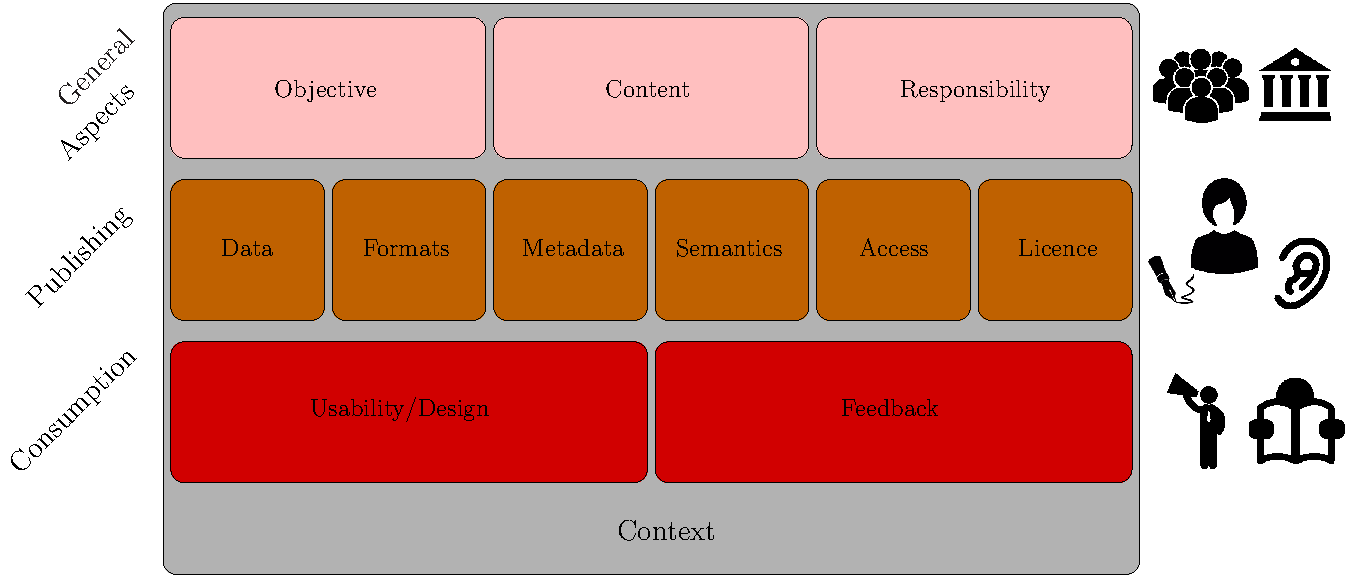
\includegraphics[scale=0.75]{images/model.pdf}
\caption[Analysis framework open budget initiatives.]{Analysis framework for open budget initiatives. The four parts -- General Aspects, Publishing, Consumption and Context -- are interconnected, and composed by several dimensions. Icons:\href{http://www.flaticon.com/authors/icomoon}{Flaticon (CC)}.}
\label{fig:framework}
\end{center}
\end{figure*}


Results from the application of this framework to 23 open budget initiatives can be seen at \url{http://bit.ly/1FNThhH}.
The goal of the evaluation is not to be extensive or to achieve statistical significance, but rather to test the model, to discover its potentials and limitations, and to gain some intuition on the domain.

The 23 initiatives were chosen considering a balance between primary (11) and secondary (12) sources. 
The sample also contains at least five initiatives strongly related to each use perspective, and considers initiatives from 6 countries plus the European Union, presented in five different idioms. Some of the analysed initiatives are listed on the \emph{Map of Spending Projects}\footnote{Available at \url{http://community.openspending.org/map-of-spending-projects/}.}.

All primary sources are maintained by the government, and most of the secondary ones are society driven. 
Among them, two initiatives were identified as maintained in partnership between government and society organizations. 
Initiatives generally display their objectives (22), but only 11 explicitly mention their intended audience. 
Also, almost all initiatives offer data for download (18), which favours transparency perspective, and more than half of them (13) make visualization available, favouring participation perspective.

Even considering the low number of initiatives evaluated, two outcomes drew the attention, regarding feedback and semantics. 
Commenting on data is allowed only in three initiatives, and the same number (but not the same ones) offers a data request form.
No reporting issues mechanisms were found, revealing a strong absence of feedback possibilities.

The lack of semantics support (only three offered it), or linkable data (again, only three had it) also may point that policy marking perspective is still far from reality. 
Ten initiatives use categories for the datasets, which at least facilitate some form of comparisons.
Regarding the use perspectives, we can state:

\noindent\textbf{Transparency:}
The main requirements for this use perspective -- data on transaction level, machine readable formats and aggregation levels -- were accomplished by most of the open budget initiatives. 
However, much work is still to be done concerning the feedback handling.
We can say that, for most of the analysed cases, stakeholders interested in auditing government and in translating data into more accessible formats are partially satisfied.

\vspace{.1cm}

\noindent \textbf{Participation:}
The requirements set for this use perspective enforced human readable formats that allow citizens without deep budget knowledge to understand data and to participate in discussions.
Slightly more than half of the initiatives present graphics, which can help quick insights over data.
Only three initiatives offer maps to visualize budget data, what is coherent to the low number of initiatives that include the location dimension (eight).
Another aspect emphasized in this use perspective was the usability and design. 
Considering the already mentioned limitations on assessing this issue, we noticed that ten initiatives use standard open source software tools. 
Although this is not the most relevant factor regarding usability, the use of standard tools favours users dealing with several open budget initiatives.
Moreover, as open source tools, the more initiatives using these tools, the better they can be developed.

\vspace{.1cm}

\noindent \textbf{Policy Making:}
The main requirements in this perspective were the use of common classifications, vocabularies and ontologies, and the possibility of linking data with other databases.
As already mentioned, semantics support was mostly absent. Comparison tools, also important in this case, were found only in three of the initiatives. 
Thus, this use perspective is still far from being realised in most of the analysed initiatives. 
All these indicate that working on standard terminologies and common conceptualizations as suggested by OpenSpending~\cite{OpenSpending} is highly desirable.

The application of the model to 23 open budget initiatives made possible to derive several conclusions related to the specific use cases.
However, it would be necessary a larger number of analysis and more iterations of the inductive-deductive approach in order be sure about the completeness of the model.

\section{Evaluating Open Data Impacts}
\label{sec:impacts}

Although mapping initiatives is a very important way of assessing the quality of published data between countries, very little is known about the final effects of these policies.
Almost a decade after the implementation in large scale of open data policies, researchers and practitioners start to pose the question: how to assess open data impacts on the society?

In order to tackle this question, a theoretical background to analyse the impact of OGD was developed by~\citeonline{Granickas2013}. 
Impacts are divided into economic, political and social, and for each of them, possible implementation issues and impact metrics are deeply discussed.
Recently, a working group was created to develop methods for assessing open data. In their first report~\cite{Caplan2014}, a draft of a framework is proposed.

Finally, a recent report run a thorough review over evidences of impacts of fiscal openness~\cite{Renzio2015}. While recognizing that there is a literature gap on testing causal effects, the most rigorous studies found a relation between open budget initiatives and the desired outcomes.

An impact evaluation and comparison between almost 30 Brazilian government transparency portals, on several administration levels, is presented by~\citeonline{Beghin2014}. The analysis was based on the 8 Open Government Principles evaluated for each portal by experts. Despite being a well defined and wide accepted model, these principles are quite general, and do not refer to specific characteristics of budget data. Moreover, they cover basically the publisher side.


\section{Open Data Value}
\label{sec:value}

Another way of assessing open data impacts is through the analysis of \emph{open data value}.
Releasing social and commercial value is cited under the main motivations for governments to publish open data (see Section \ref{sec:why}).
Thus, it is necessary to understand the chain of value addition over data, and specifically what activities may add value for data.
\citeonline{Jetzek2013} developed a conceptual model of OGD value generation, where enabling factors lead to value generation mechanisms which should finally release social and commercial value. 

\citeonline{Attard2016} proposed a Value Creation Assessment Framework, which profits from previous works, and extends some aspects.
The framework walks through the complete Government Data Life Cycle Processes, namely: data creation, harmonisation, publishing, interlinking, exploitation and curation, and defines implementation and impact aspects related to each stage.

%\section{Open Data and Participation}

%Enabling citizen participation in democracy is one of the mentioned motivations for using open data.
%The reasoning behind it is that the release of open data makes citizens more informed, and thus are more able to participate in public decisions.
%One of the most famous processes of citizen participation is the Participatory Budget.

%\begin{itemize}
%	\item Origins of PB, and impact analysis in Brazil~\cite{Goncalves2014}
%	\item Definitions: \cite{Zhang2013}
%	\item Description of Cuiabá case: \cite{Borges2012}
%	\item PB critics: \cite{Masser2013}
%	\item 10 reasons to implement: \cite{Nitschke2013}
%	\item Comparisson between online and offline PB: \cite{Peixoto2009}
%	\item Conditions for participation: \cite{Addor2012}
%	\item Budget data publishing process, including feedback: \cite{Alexopoulos2014}
%	\item Deep analysis about PB, focusing on the poor \cite{TheWorldBank2001}
%	\item Literature review, definitions and a model to analyse PB \cite{Miller2014}
%\end{itemize}

%As a complementary approach, we also interviewed two domain experts: 
%\begin{itemize}
%	\item a government employee who activeley supported a PB process
%	\item and the director of a transparency oriented Civil Society Organization (CSO)
%\end{itemize}


%%
%#############################################
\subsection{Introduction}
%#############################################
The literature about participatory budget is vast. The possibility of enhancing democracy through direct participation of citizens in a crucial political decision, i.e., budget allocation, attracted the attention of researches since the first well known experiences in Porto Alegre, in the 1980 decade.

Since then, several implementations all over the world were experimented, with many successful and fail stories. The use of online tools, both for supporting PB process and for publishing related datasets was also part of the more recent experiences.

In this review, we try to picture the state of art of PB, pros and cons and the mechanisms used, with a special focus on the online ones. The final objective is to detect how online information systems can help build a more effective participation, both higher and better informed, to produce better outcomes.

%#############################################
\subsection{Summary of Analysed of Works}
%#############################################
\begin{itemize}
	\item Origins of PB, and impact analysis in Brazil~\cite{Goncalves2014}
	\item Definitions: \cite{Zhang2013}
	\item Description of Cuiabá case: \cite{Borges2012}
	\item PB critics: \cite{Masser2013}
	\item 10 reasons to implement: \cite{Nitschke2013}
	\item Comparisson between online and offline PB: \cite{Peixoto2009}
	\item Conditions for participation: \cite{Addor2012}
	\item Budget data publishing process, including feedback: \cite{Alexopoulos2014}
	\item Deep analysis about PB, focusing on the poor \cite{TheWorldBank2001}
	\item Literature review, definitions and a model to analyse PB \cite{Miller2014}
\end{itemize}

As a complementary approach, we also interviewed two domain experts: 
\begin{itemize}
	\item a government employee who activeley supported a PB process
	\item and the director of a transparency oriented Civil Society Organization (CSO)
\end{itemize}

%#############################################
\subsection{Origins}
%#############################################

\cite{Goncalves2014} describes the first PB experiences in Brazil in the context of the country's redemocratization. After 20 years of military dictatorship, in the late 1980's, many efforts were driven in order to decentralize the public administration, from the federal level to the cities. In this context, the Workers Party was created, and as soon it elected the first mayors, PB was implemented as a symbol of direct democracy and transparency, as oposed to the previous regime.

Still according to \cite{Goncalves2014}, in Porto Alegre, the most cited PB showcase, the number of participants raised from around 1000, in 1989, to around 20,000 in the late 1990/early 2000. The alleged reason is that the people demands were realy undertaken by the governments.

According to \cite{Miller2014}, in 2010 nearly 1,500 municipalities worldwide adopted PB.

%#############################################
\subsection{PB Cycle}
%#############################################
According to~\cite{Giacomoni2007}, the classical Budget cycle comprises 4 phases:

\begin{enumerate}
\item Elaboration and presentation
\item Legislative authorization
\item Programming and execution
\item Evaluation and controll;
\end{enumerate}


Figure~\ref{fig:POA} shows the workflow used in Porto Alegre.

\begin{figure}[h]
\begin{center}
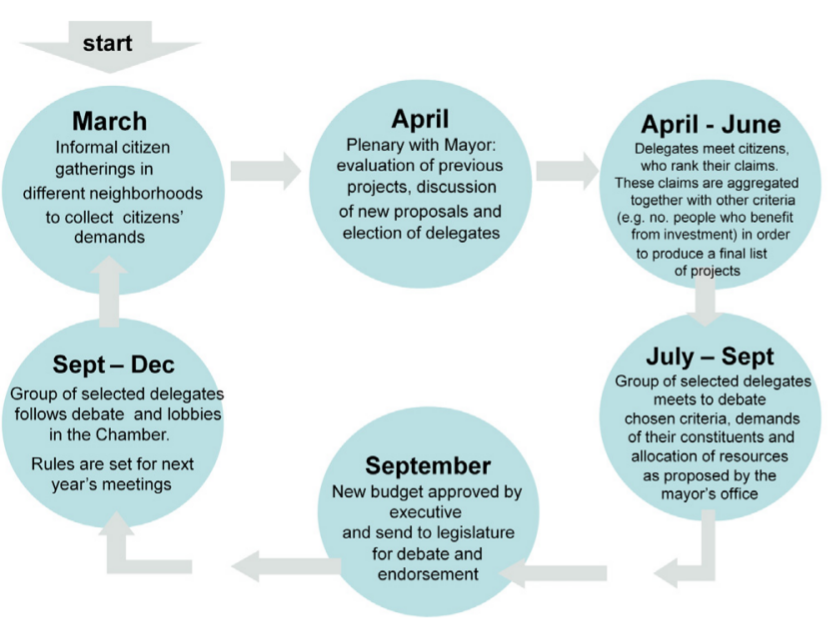
\includegraphics[scale=0.35]{images/portoalegreworkflow.png}
\caption{Workflow of Porto Alegre's PB. Author: \cite{Goncalves2014}\label{fig:POA}}
\end{center}
\end{figure}

\cite{TheWorldBank2001} summarizes four fases, illustrated in Figure~\ref{fig:WB}:
\begin{enumerate}
\item Budget formulation
\item Budge analysis
\item Budget expenditure
\item Performance monitoring
\end{enumerate}

\begin{figure}[h]
\begin{center}
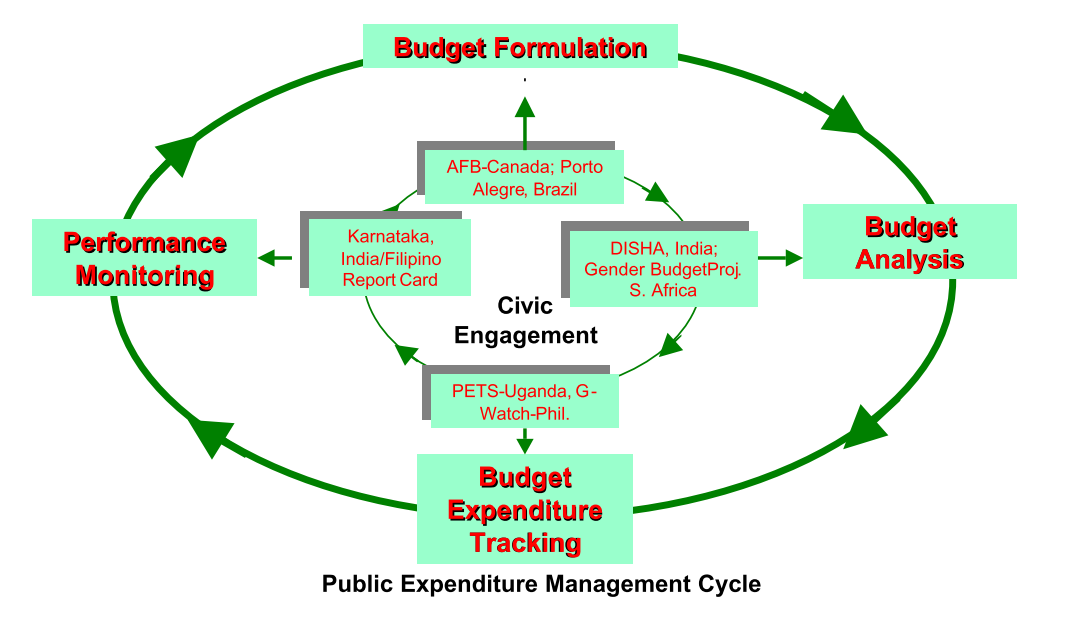
\includegraphics[scale=0.35]{images/cycle_WB.png}
\caption{Generic PB Workflow. Author: \cite{TheWorldBank2001}\label{fig:WB}}
\end{center}
\end{figure}



%#############################################
\subsection{Definitions}
%#############################################

\cite{Zhang2013} proposed some definitions on this field:

\noindent\textbf{Participatory budgeting} refers to a situation in which government officials invite citizens' input during the budget process and allows citizen to influence budgetary decisions (Zhang \& Yang, 2009).

\noindent\textbf{Mechanisms of participatory budgeting} refer to any tools provided by government for citizen involvement, including public hearings, citizen surveys, telephone hotlines, citizen advisory boards, focus group, as well as encouraging citizens to speak about budget in regular meetings, posting budget materials on the Internet, working with local media to highlight citizen comments during deliberation, and so on.

These mechanisms are of two kind:

\noindent\textbf{One way mechanisms:} Coordinating with the local media, such as TV and radio, to invite the public comments; Citizen surveys about spending priorities and needs through mail, Internet or telephone; Posting budget materials on Internet sites; Hotlines for citizens to provide suggestions or comments.

\noindent\textbf{Two way mechanisms:} Public budgetary hearings; Forums or workshops open to citizens during budget preparation; Opportunities for citizens to speak at regular meetings; Citizen advisory boards; Focus groups.
We define “two-way communication” as a process of face-to-face interaction between citizens and government officials in which citizens are provided with an opportunity to directly raise concerns and discuss them with government officials. Two-way communication can nurture social learning and collaborations between citizens and government because it enables stakeholders to respect and listen to one another’s opinions, and allows competing perspectives to be aired and considered before decisions are made (King, Feltey, \& Susel, 1998; Roberts, 2004).

In his review, \cite{Miller2014} also collected a number of other definitions. They also point some literature confusions, specially in the US. One of the points is that labelling the above mentioned one way mechanisms as PB ``eliminates from participatory budgeting what is distinctive, valuable, and potentially transformative".

%#############################################
\subsection{Motivations for implementing PB}
%#############################################

In a sort of ``marketing paper", \cite{Nitschke2013} proposes 10 reasons for public administrations to addopt PB:

\begin{enumerate}
\item Greater acceptance of priorities that are better harmonised
\item Making administration more efficient by integrating citizens’ knowledge
\item Increasing problem-solving capabilities
\item Greater cost awareness
\item Mobilising citizen engagement
\item Reducing political disenchantment and disillusionment with political parties
\item Fostering democracy
\item Supporting modernisation processes within the administration
\item Improved image for the local authority
\item Risks do exist, but they can be successfully managed
\end{enumerate}

As we will see in the next section, many of these ``benefits" can turn into impediments if not well implemented.

The political conditions for a sucessfull participation process are object of a political science oriented study by \cite{Addor2012}. After deeply analysing two experiences - not only of PB, but of wider participation practices - he formulated seven factors that influenced on the establishment and strengthening of the participator practices:

\begin{enumerate}
\item Politicisation of the society
\item Transformation of the reality
\item Permission of the utopia
\item Basis organization
\item Exchanges with other experiences
\item Involvement of the state
\item Formalization of the political commitment
\end{enumerate}

%#############################################
\subsection{Criticisms on PB}
%#############################################

\citeonline{Masser2013} summarized common criticisms to PB, specially in the German context. He considered that the first wave of PB experiences in the country failled: ``The original objective of involving citizens in the complex process of municipal budget formulation was not achieved, and has since been abandoned. Nowadays, it is only collections of proposals for measures and (investment) projects, or voting procedures on proposals made by policymakers and administrators, that operate under the label ‘participatory budgeting’."

The first argument is about \textbf{low participation}. ``The question therefore arises of whether the measures identified through PB possess sufficient legitimacy to warrant their adoption by democratically elected local councils."

This leads to a second argument that states the \textbf{under representation} of the society in PB practice.

Another argument lies in the \textbf{high cost of participation}, which is a consequence of the low participation. ``The low figures for participation raise another problem:  how sustainable is citizen participation through PB? In many cases we can see that PB has already been discontinued. The question as to whether ‘participatory budgeting’ as a whole is gradually fading away seems warranted. This is because, as with employee suggestion schemes, in PB fresh ideas are not forthcoming every day. In fact, there is a risk that the debate will keep returning to many similar proposals or even the same ones."

\textbf{Conclusions:}
The original intention of integrating citizens closely into the budget formulation process has not been realised;

The influence that citizens wield in this procedure is limited, because only a few proposals made by a few citizens have a chance of being realised, even though each and every citizen does have an opportunity to influence things by prioritising and voting on the proposals;

The fact that the influence of citizens is not all that significant might also benefit PB, in that members of local councils might then be far more willing to embrace this tool. 

There remains a trend toward PB. The Fifth Status Report on ‘Participatory Budgeting in Germany’ published in March 2012 identifies 21 newly active municipalities that are conducting PB. This makes a total of 115 active local authorities that are either conducting PB or have at least done so within the last two years.

%#############################################
\subsection{Some current PB cases}
%#############################################

\subsubsection{\href{http://pbnyc.org/}{New York}}
``New York City is experiencing a new kind of democracy. Through Participatory Budgeting, residents of twenty-four Council Districts across the City are directly deciding how to spend \$25 million of taxpayer money. From September 2014 to April 2015, community members are exchanging ideas, working together to turn ideas into project proposals, and voting to decide what proposals get funded."

\subsubsection{\href{http://cambridgema.nationbuilder.com}{Cambridge}}
``In December, community members shared over 380 ideas for projects to improve Cambridge.  From January-March, 40+ volunteer Budget Delegates prioritized and developed those ideas into 20 concrete project proposals for community members to vote on. Over 2,700 Cambridge residents age 12 and older voted online and at events around town from March 22-28, 2015 to decide which projects the City should fund."

\subsubsection{\href{https://budgetparticipatif.paris.fr}{Paris}}
In Paris, the major selected 15 projects and made \$20 million Euros for that. Over 40,000 people participated, being 40\% online. Among the 15, nine project were chosen to be developed in 2015. This year, almost 20,000 people proposed over 5,000 ideas.

\subsubsection{\href{http://planejasampa.prefeitura.sp.gov.br/}{São Paulo}}
In São Paulo, the Planning and Budget Participatory Cycle envisages a four year cycle, and is based on fisical goals. Direct participation resulted in 123 goals. 11,000 people formulated (physically) 9,489 suggestions, which resulted in the goals. There were also 2 hacker meetings, with 100 presential participants. A tool was developed for monitoring the goals by the elected councillors.

\subsubsection{Other related links}
\begin{itemize}
	\item \href{http://pbnetwork.org.uk/}{PB Network (UK)}
\end{itemize}

%#############################################
\subsection{Profile of the Participants}
%#############################################
\cite{Masser2013} reports that ``The vast majority are middle-aged men who left school well-qualified and now have well-paid jobs". 

On the other hand, \cite{Goncalves2014} reports that ``data collected at the participatory budgeting forums in Porto Alegre, in 2002, reveal that the participatory assemblies tend to concentrate a higher proportion of (i) women, (ii) elders and retired workers, (iii) married people, (iv) non-qualified workers, (v) people with lower average income, (vi) higher rates of associative life, and (vii) stronger identification with the Workers’ Party ideology than the city’s average dweller."

\cite{Peixoto2009} also reports advanced age and lower socio-economic background.


%#############################################
\subsection{The role of online tools in PB}
%#############################################
The use of online tools for PB was described by \cite{Peixoto2009}. According to him, ``evidence suggests that the online forum was, overall, an environment of rational, argumentative and reflective debates where active participants would persuade and be persuaded of the importance of one public work over another and where readers - in larger numbers - could be informed on concurrent perspectives."

In the voting for priorities, as expected, the participation was higher than the standard PB. It was noticed that people tend to vote locally, i.e., to choose works near their residences. This is also somehow expected, as the original target of PB is to descentralize power and let communities decide what is better for them.

``One element that was considered important for the success of the e-PB was the city’s communication campaign, which focused on the initiative and its novelty factor.''

Finally, the author considers that online PB should be just a complementary action to be taken together with tradiciontal PB. 


%#############################################
\subsection{Linking Budget Planning with final result}
%#############################################
As pointed by several works \cite{Addor2012, Miller2014, TheWorldBank2001, Borges2012}, a crucial element for raising participation is to guarantee that the decisions taken by the citizen council will be really implemented. Although this is a quite obvious conclusion, the disconnection between what is decided and what is implemented has been pointed to be the reason of several PB experiences (\cite{Borges2012}).

One of the interviewees was a government employee responsible for coordinating a PB process in a medium size city in Brazil. The process of collecting citizen demands was successful, with high participation of citizens and community leaders. All PB assemblies had the presence of at least four government representatives, so that proposals could be discussed with the ones responsible to implement it. 

However, the final result was modified by the legislative, and not totally implemented in the following year. In second year of PB, a new mayor was elected, and PB received less attention. The government officials stopped attending the meeting, and PB failed.

Another big issue pointed by the interviewee was the lack of transparency inside government. In his opinion, government information systems suffer from a lack of integration that seriously compromises transparency. With an integrated information approach, citizens could easily follow a demand from budget planning until the execution, and even assess specific targets, for example, more kids on the school or decrease of illness caused by lack of sewage.

The second interviewee, member of a transparency oriented SCO, reported the same scenario of decoupled systems in another medium size city in Brazil, which deeply hinders transparence. A mayor change altered positively the scenario, but crucial measures, as online procurements, were still no implemented. He calls the attention also for a transparency in the councils, because many times, council members may be representing private interests, or not representing anything at all.

One aspect point by this domain expert is the financing of participation. He pointed that, many times, counting only on voluntary efforts may not be enough to audit the government. On the other hand, possible financiers, as commercial association, may have different interests in relation to transparency.



%#############################################
\subsection{Open Budget Experiences}
%#############################################

In the specific field Open Budgets, the experience of three countries was recently reported: \href{http://fiscaltransparency.net/wp-content/uploads/2015/03/GIFT-Kenya-Webinar-Deck.pdf}{Kenya}, \href{http://fiscaltransparency.net/wp-content/uploads/2015/03/GIFT-MEX-TP-Webinar-Deck.pdf}{Mexico} and \href{http://fiscaltransparency.net/wp-content/uploads/2015/03/GIFT-Chicago-NYC-Webinar-Deck.pdf}{Chicago and NYC}.

A \href{http://pt.slideshare.net/jwyg/open-budget-data-a-landscape-analysis}{landscape analysis} with several definitions and cases was also presented.

%#############################################
\subsection{Software Tools}
%#############################################

\noindent\textbf{\href{http://budgetallocator.com/}{Budget Allocator}: } This online tools is a one way mechanism of budget participation. It offers the citizen the chance to submit a number of choices - increase, decrease or maintain police expends, for example, or build a pool, a school or a hospital - and some comments over it. If your choices are over budget, the system warns about a possible tax increase. The licence costs between U\$200 and U\$2000.

\noindent\textbf{\href{http://www.engagedata.eu/}{Engage}: } With this platform, users are able to submit, acquire, search and visualize diverse, distributed and derived Public sector datasets from all the countries of the European Union. A special focus is given on the feedback loop. The tool allows discussion and suggestions on specific datasets, as described in~\cite{Alexopoulos2014}.

\noindent\textbf{\href{https://www.participare.io/}{Participare}: } `` It provides an easy to use, do-it-yourself like, Participatory Budgeting platform capable of adapting to the best practices as well as local specificities."

\noindent\textbf{\href{https://docs.google.com/spreadsheets/d/1f1iHQFGIc5MmmzdRVkBk6hXyrrLnoNP4aaOM9w85agw/}{OpenSpending List}: } List of 60 softwares which support some kind of participation.

%#############################################
\subsection{Some conclusions}
%#############################################
\begin{itemize}
\item Participatory budget is, most of all, a political action. The only possibility for it to work properly is to be fully and truly supported by the government;
\item Given the political support, it is also important to 'close the loop', i.e., connect the ellected demands with the monitoring of the concrete results and the high level targets;
\item Online tools have to be combined with presential strategies, and must cover the whole budget cycle - from definition to target monitoring.
\end{itemize}



\section{Problems of Open Data}
\label{sec:problems}
\cite{Roseira2016}

The vast majority of research about open data assumes that publishing public data in open formats will bring mostly good impacts.
In this sense, two works from the same research group made an in depth research on the negative sides of open data.

In the first one, \citeonline{Zuiderwijk2012} analysed the socio-technical impediments that hinders the use of open data via literature review, interviews and workshops.
As a result, 118 impediments were summarized in 10 categories: availability and access, find ability, usability, understand ability, quality, linking and combining data, comparability and compatibility, metadata, interaction with data provider and opening and uploading.

The second paper focuses on the possible negative effects that governments may face on opening data. \citeonline{Zuiderwijk2014a} conducted several interviews with public servants and data archivists to find out which negatives effect they were concerned with.
As a result, 16 negative effects were listed, for example: ``risk of violating legislation by opening data'', ``privacy can be violated unintentionally'', ``misinterpretation and misuse'', ``not citizens but others profit from open data'' and ``wasting resources to publish invaluable data''.
It is interesting to note the question of data value also appearing here.
In fact, methods for determining the value of data for users could help publishers selecting in which data should they put efforts.

Regarding the risk of privacy violation, two recent episodes attest that these concerns should really be taken into account.
As reported by \citeonline{Hern2014}, the opening of taxi trips data by the city of New York allowed the identity of drivers to be discovered, and in some cases, even the passengers could be identified.
In a similar situation, the release of film ranking data allowed not only the identity of users to be unveiled, but also their political orientation, religious views or sexual orientation.
In both cases, the attempt to anonymise data failed.

\citeonline{Parycek2016} interviewed 

\subsection{The Missing Focus on Use of Open Data}

Another aspect revealed by~\citeonline{Zuiderwijk2014a} is the lack of informations interest about the actual use of open data: ``The interviewees stated that they do not have much more information about how the open data have been used than the number of downloads''.

One of the few works dealing with this subject was written by~\citeonline{Davies2012}. According to the author, ``The gap between the promise and reality of OGD re--use cannot be addressed by technological solutions alone''.
Thus, he raises the necessity of considering human factors that affect the use or no use of data.
In this paper, a Charter of Open Data Engagement is proposed, aiming to derive a parallel of the Five Stars of Open Data~\cite{Berners-Lee2010}, but from the users point of view.

The five stars of open data engagement are~\cite{Davies2012}:

\begin{itemize}
	\item Be demand driven
	\item Put data in context
	\item Support conversation around data
	\item Build capacities, skills and networks
	\item Collaborate on data as a common resource
\end{itemize}

In the same work, Davies criticizes the so called ``application fallacy''.
According to him, the narratives about OGD assume that someone will develop an application to consume and visualize data.
However, in his master thesis,~\citeonline{Davies2010} ran a survey with 55 instances using OGD from data.gov.uk, which revealed that in most of the cases facts are directly identified within datasets.
Data is then used to base discursive reports, or to generate derivative datasets.

\citeonline{Davies2010} describes five ways of using open data. Figure~\ref{fig:opendatause} shows the categories, and the number of cases gathered on the survey.

\begin{figure}[h!]
\begin{center}
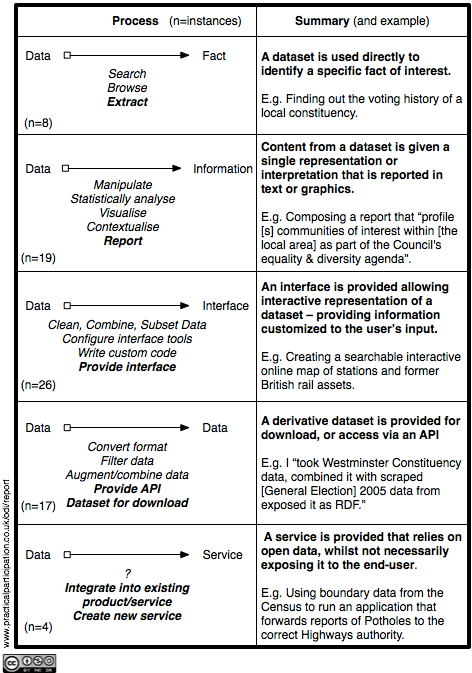
\includegraphics[scale=0.6]{images/Data-Schematic-FiveTypes}
\caption[Different uses of data, with process, summary and examples.]{Different uses of data, with process, summary and examples. For each type, the number of instances (n) found is detailed. Source: \citeonline{Davies2010}}
\label{fig:opendatause}
\end{center}
\end{figure}

As a contribution for future research, author cites some challenges in the social and technical fields.
The priority, according to him, is to understand the process that occurs between data publishing and its use in a determined application.
Through this understanding it will be possible to overcome the barriers for use of data.
Moreover, it is necessary to explore the existent political structures, so that the informations brought by data can effectively generate social changes.
Finally, the broader challenge is to better understand the user point of view.
The greatest technical challenge associated is to create tools that not only show data, but that support discussion and interaction around them.

\subsection{Open Data Capacities and Data Divide}
\label{sec:datadivide}

Still according to~\citeonline{Zuiderwijk2012}, two of the broad categories of open data impediments are ``Usability'' and ``Understand ability'', under which 33 problems were mapped.
Under these, we can list at least seven directly related to the lack of capacities from the user side deal with data:

\begin{itemize}
	\item Data are not understandable for the general public (e.g. related to jargon). 
	\item No explanation of the meaning of data. 
	\item Lack of knowledge about how to interpret the data. 
	\item Lack of skills and capabilities to use the data. 
	\item Lack of statistical knowledge.
	\item Lack of (domain) knowledge about how to treat the data. 
	\item Expert advice is needed to use the data.
\end{itemize}

\citeonline{Zuiderwijk2014a}, based on several interviews with government officials, affirm that this lack of capacities in using data may lead to negative effects in open data: 

\begin{citacao}
(...) stakeholders do not profit equally from the opening of data. The use of open data is complex, time-intensive and might require certain skills to find, understand and use data. This results in a high threshold for ordinary citizens to make use of the data. Instead journalist and lobbyist have more time and are often skilled in making use of the data. As such open data can be used by certain groups to strengthen their position, instead of creating a level playing field~\cite{Zuiderwijk2014a}.
\end{citacao}

Inequalities in access to data is starting to raise concerns for those who, for many years, studied the inequalities in access to ICTs.
Micheal Gurstein is probably the pioneer in calling attention for this and coining the term \emph{data divide}: 

\begin{citacao}
Efforts to extend access to “data” will perhaps inevitably create a “data divide” parallel to the oft–discussed “digital divide” between those who have access to data which could have significance in their daily lives and those who don’t \cite{Gurstein2011}.
\end{citacao}

A data divide between countries is also mentioned as one of the conclusion of the Open Data Barometer project.
\citeonline{Davies2015} states that the data divide between countries has grown from the first edition of the evaluation, in 2013, to the second one, in 2014.
Countries are clustered into four classes to define their stage in implementing open data policies: High capacity, Emerging and advancing, Capacity constrained and One sided initiative.

Another important publication which shows concerns with data divide is the report by the~\citeonline{DataRevolutionGroup2014}: ``There are huge and growing inequalities in access to data and information and in the ability to use it''.
The group hosted by the United Nations warns that ``Without immediate action, gaps between developed and developing countries, between information-rich and information-poor people, and between the private and public sectors will widen, and risks of harm and abuses of human rights will grow.''


\section{Linked Data towards Semantic Organization of Open Data}

\label{sec:LOD}

One of the strategies for adding value to data is the interlinking with other datasets.
As described by~\citeonline{Attard2016}, Data Interlinking is one of the steps in data cycle that involves value creation.
The value creation techniques at this step are Link Discovery, Data Interlinking and Data Integration.
``Missing links between data'' is also cited as a problem for the use open data.
\citeonline{Zuiderwijk2012} summarized 9 impediments under the category ``Linking and combining data'', such as ``Data cannot be linked to other data'' or ``No unique identifiers are available''.

Since the publication of the paper \emph{Linked Data - Design Issues}~\cite{Berners-Lee2006}, a new paradigm over online data organization is being pushed: Linked Open Data, better known by its acronym LOD.
The main inspiration is exactly the problem of interlinking heterogeneous data over the Web.

\citeonline{Berners-Lee2006} formulates four basic rules that establishes best practices for linking data: 

\begin{enumerate}
	\item Use URIs as names for things;
	\item Use HTTP URIs so that people can look up those names;
	\item When someone looks up a URI, provide useful information, using the standards (RDF*, SPARQL);
	\item Include links to other URIs. so that they can discover more things.
\end{enumerate}

Thus, a dataset is represented as Linked Open Data if every data unit is identified through dereferenceable HTTP URIs, which should by linked to another in form of a graph.
Following the RDF standard, the graph is composed by several connected triples, describing the connection between a subject and an object through a predicate.

The implementation of these rules in several datasets forms an interlinked graph database connected through common elements which is known as LOD Cloud.
The last update from the LOD Cloud platform\footnote{Available at \url{http://lod-cloud.net/}.}, in 2014, considers 1014 datasets, using 649 vocabularies as RDF, RDFS, Friend-of-a-friend, Dublin Core and others.
Most of the datasets are belong to the category Social Web (51\%), while Government data represents 18\%. The remaining datasets are labelled under Publications (10\%), Life sciences (8\%), User-generated content (5\%), Cross-domain (4\%), Media (2\%) and Geographic (2\%).

Linking data from different datasets over a big virtual cloud is not the only main benefit from the Linked Open Data paradigm.
Representing data using shared, linked and standardized metadata can also enable the concept of \emph{Semantic Web}.
The idea that computers can understand the meaning of data and documents on the web was already present in the early 2000's, as shown by~\citeonline{Berners-Lee2001}. In this paper, the authors imagine a scenario where several agents present in different devices develop a meaningful communication to solve a problem: setting an appointment with a specialist doctor respecting the agenda and location constraints of several people.

For this scenario to become real, a computer readable definition of how the world works must be developed.
This is the main objective of the information science \emph{ontologies}.
In the words of Barry Smith, ``ontology as a branch of philosophy is the science of what is, of the kinds and structures of objects, properties, events, processes and relations in every area of reality''\cite{Smith2003}.
On the information science field, ontologies came to solve the Tower of Babel problem: different systems with their own concept and relationships definitions wanting to exchange data.
According to~\citeonline{Smith2003}, ``an ontology is a formal theory within which not only definitions but also a supporting framework of axioms is included''.
These axioms should explain for computers implicit rules present in the spoken language, e.g., that \emph{a niece is a daughter of a person's brother or sister}.

Currently there are several widely used ontologies, either context specific, as \href{http://www.imdb.com}{IMDb} for movies, or \href{http://aims.fao.org/skosmos/agrovoc/en/}{Agrovoc} for agriculture, of foundational ontologies as \href{http://www.loa.istc.cnr.it/old/DOLCE.html}{DOLCE} or \href{http://ontology.com.br/}{UFO}.
Though less descriptive and formal than ontologies, several vocabularies are being used to describe semantic content on the Web.
Currently, one of the most successful vocabularies is \href{http://schema.org}{Schema.org}, sponsored by Google, Microsoft, Yahoo and Yandex, which claims to be present in over 10 million websites.

On the OGD field, Linked Open Data is still on its first steps.
UK's open data portal presents currently 216 datasets in RDF format, which represents 0.93\% of all datasets published in data.gov.uk.
In his turn, US's data.gov presents 7534 or 3.87\% datasets in RDF.


\section{Conclusions}

In this chapter, an overview about Open Data was presented.
We highlighted some aspects as definitions and main research problems currently posed.
For a more complete view on Open Data, please consult the following selected bibliography:
\begin{itemize}
\item \emph{Community Informatics and Open Government Data}, by~\citeonline{Davies2012a}
\item \emph{Open Government Data: The Book}, by~\citeonline{Tauberer2014}
\item \emph{A Systematic Review of Open Government Data Initiatives}, by~\citeonline{Attard2015}
\end{itemize}

This chapter was written basically after a literature research.
In the next chapter, we also take conclusions about open data based on the impressions after giving open data classes for social movements activists.

